\documentclass[11pt]{amsart}
%\documentclass[11pt]{report}
\usepackage[toc,page]{appendix}
\usepackage{float}
\usepackage{mathtools}
\usepackage{geometry}        % See geometry.pdf to learn the layout options.
\geometry{a4paper}           % ... or a4paper or a5paper or ...
%\geometry{landscape}        % Activate for for rotated page geometry
%\usepackage[parfill]{parskip} % Activate to begin paragraphs with empty line
\usepackage{graphicx}
\usepackage{amssymb}
\usepackage{epstopdf}
\DeclareGraphicsRule{.tif}{png}{.png}{`convert #1 `dirname #1`/`basename #1 .tif`.png}
\graphicspath{ {images/} }

\renewcommand{\familydefault}{\sfdefault}
\newcounter{defctr}

\title{SDBM\_Tree Balanced Tree Database System (Compendium)}
\author{Kees-Jan Hermans}
%\date{}                     % Activate to display a given date or no date

\begin{document}
\maketitle

This document contains a description of sdbm\_tree, a C library that
implements a balanced database tree with a focus on simplicity,
integrity and openness.

\vspace*{3\baselineskip}

%Image
\begin{figure}[H]
\centering
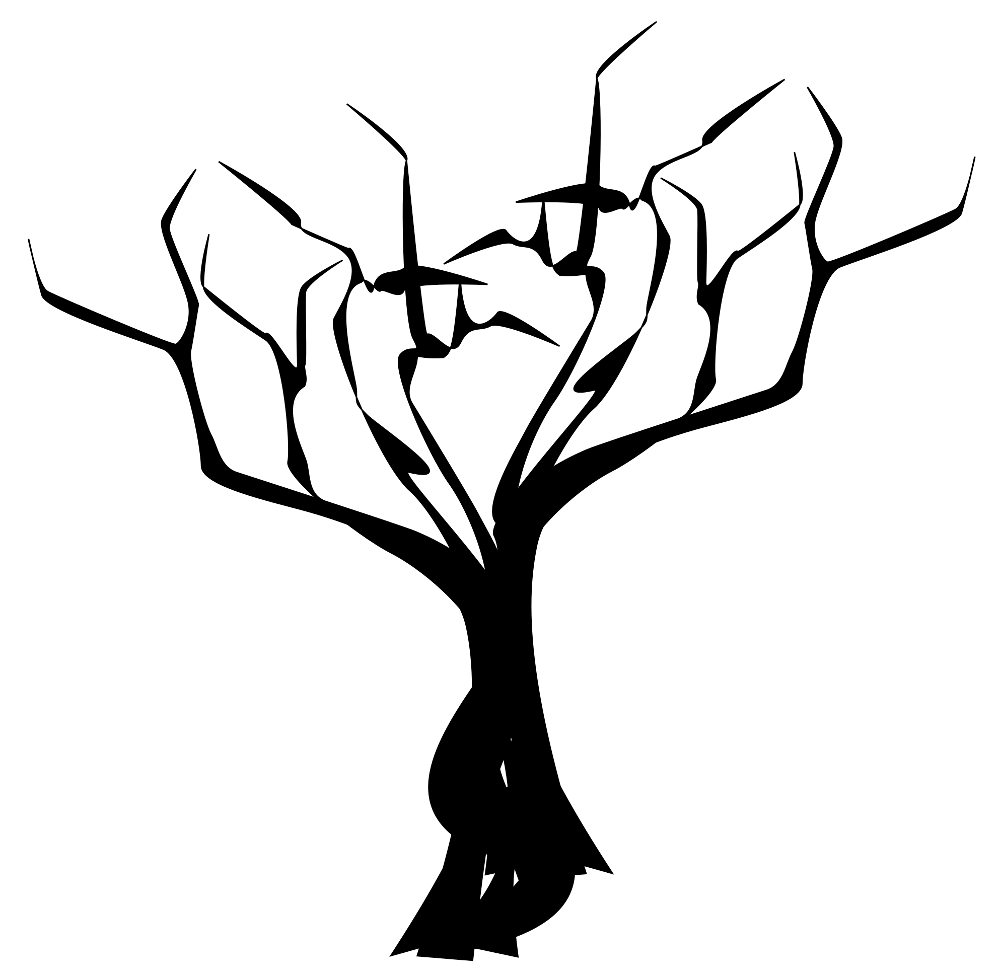
\includegraphics[width=100mm]{tree.png}
\end{figure}

\vfill

\begin{table}[]
\centering
\begin{tabular}{ll}
Accompanies release & \input{../../release} \\
Author &  Kees-Jan Hermans / kees.jan.hermans@gmail.com \\
Classification & - \\
Generated on & \today \\
\end{tabular}
\end{table}

% Accompanies release: \input{../../release}
% 
% Author: Kees-Jan Hermans / kees.jan.hermans@gmail.com
% 
% Classification: -
% 
% Generated on: \today
\newpage
\tableofcontents

\setlength{\parindent}{4em}
\setlength{\parskip}{1em}

\newpage

\section{Introduction}

blah blah blah


%% all the rest of the content

\newpage
\section{Colofon}

%\chapter
%\addtocontents{lof}{\vspace*{-10pt}}
%\addtocontents{lot}{\vspace*{-10pt}}

%\setlength{\cftbeforesecskip}{0pt}
%\setlength{\cftbeforeXskip}{0pt}
\listoftables

\newpage

% \listoffigures

\input{bib.tex}

\newpage
\begin{appendices}

\section{Functions}

\newpage
\subsection{td\_ar\_list}
\subsubsection{Declaration} Function prototype:

\begin{verbatim}
extern
int td_ar_list
  (td_t* td, int longform);
\end{verbatim}

\subsubsection{Description}



\subsubsection{Parameters}
\subsubsection{Returns}
\subsubsection{Called by}


\newpage
\subsection{td\_ar\_scan}
\subsubsection{Declaration} Function prototype:

\begin{verbatim}
extern
int td_ar_scan
  (char* path, td_t* td);
\end{verbatim}

\subsubsection{Description}



\subsubsection{Parameters}
\subsubsection{Returns}
\subsubsection{Called by}


\newpage
\subsection{td\_ar\_unpack}
\subsubsection{Declaration} Function prototype:

\begin{verbatim}
extern
int td_ar_unpack
  (td_t* td);
\end{verbatim}

\subsubsection{Description}



\subsubsection{Parameters}
\subsubsection{Returns}
\subsubsection{Called by}


\newpage
\subsection{td\_checksum\_create}
\subsubsection{Declaration} Function prototype:

\begin{verbatim}
extern
void td_checksum_create
  (void* mem, unsigned length, unsigned* checksum);
\end{verbatim}

\subsubsection{Description}


 ingroup btree\_private

 Creates a checksum of a piece of memory.
 Does this using the FNV-1a algorithm, which is 64-bit, and
 must be reduced to sizeof(unsigned). So it is a variety of FNV.

 code

   hash = FNV\_offset\_basis
   for each byte\_of\_data to be hashed
        hash = hash XOR byte\_of\_data
        hash = hash × FNV\_prime
   return hash

 endcode

 param[in] mem Non-NULL pointer to the beginning of the memory
 to be checksummed.
 param[in] length Size of the memory to be checksummed.
 param[out] checksum On return, contains the checksum of the memory piece.
 

\subsubsection{Parameters}
\subsubsection{Returns}
\subsubsection{Called by}


\newpage
\subsection{td\_checksum\_verify}
\subsubsection{Declaration} Function prototype:

\begin{verbatim}
extern
int td_checksum_verify
  (void* mem, unsigned length, unsigned checksum);
\end{verbatim}

\subsubsection{Description}

 
 ingroup btree\_private

 Verifies a checksum of a piece of memory.

 param[in] mem Non-NULL pointer to the beginning of the memory
 to be checksummed.
 param[in] length Size of the memory to be checksummed.
 param[in] checksum The checksum to verify.

 returns Zero when the piece of memory is verified by the checksum.
 TDERR\_CHECKSUM on failure.
 

\subsubsection{Parameters}
\subsubsection{Returns}
\subsubsection{Called by}


\newpage
\subsection{td\_claim}
\subsubsection{Declaration} Function prototype:

\begin{verbatim}
extern
int td_claim
  (td_t* td, int contiguous, unsigned* off, unsigned* size);
\end{verbatim}

\subsubsection{Description}


 ingroup btree\_private

 Claims an amount of resources.
 While iterating through the linked list
 of empty chunks, fills up a little table denoting the fittingness of
 this chunk to be used.  Perfect fits are used immediately, while
 not-so-perfect fits fill up the fitness table.  In the end, when either
 the table is full or the end of the list has been reached, it makes a
 choice for the nicest record of the table, and uses the data in this
 record to make changes.

 param td Non-NULL pointer to the initialized td\_t structure.
 param contiguous Whether or not the value of *size must be met whole.
 param off Returns the offset on success
 param size Filled with requested size on calling, filled with granted
 size on return.  NB. The requested size must be the full amount of space
 requested, not diminished with chunk- or keyheader sizes.

 returns Zero on success, TDERR\_SPACE when no piece can be found, or
 any of the errors of the underlying functions.

 par NB:
 This function assumes that the header will be written again
 when this function returns successfully.
 

\subsubsection{Parameters}
\subsubsection{Returns}
\subsubsection{Called by}


\newpage
\subsection{td\_compare}
\subsubsection{Declaration} Function prototype:

\begin{verbatim}
extern
int td_compare
  (td_t* td, const tdt_t* key1, const tdt_t* key2, int partial, void* arg);
\end{verbatim}

\subsubsection{Description}


 ingroup btree\_private

 In-house comparison call-back function.

 Compares to keys, potentially partially.
 If not partially, compares like memcmp().
 If partially, only until the length of key1.

 param td Non-NULL pointer to an initialized btree structure. 
 param key1 Non-NULL pointer to an initialized tdt.
 param key2 Non-NULL pointer to an initialized tdt.
 param partial Boolean. Whether or not partial matches are allowed.
 param arg Callback API user-provided argument.
 (Unused in this implementation).

 returns Zero when (partially) equal, smaller than zero when key1 is
 considered smaller than key2, greater than zero when key1 is considered
 greater than key2.
 

\subsubsection{Parameters}
\subsubsection{Returns}
\subsubsection{Called by}


\newpage
\subsection{td\_debug}
\subsubsection{Declaration} Function prototype:

\begin{verbatim}
extern
int td_debug
  (td_t* td);
\end{verbatim}

\subsubsection{Description}


 ingroup btree

 Debugs the structure and contents of a btree to stderr.

 param td Non-NULL pointer to an initialized btree structure.

 returns Zero on success, or a TDERR\_* value on error.
 

\subsubsection{Parameters}
\subsubsection{Returns}
\subsubsection{Called by}


\newpage
\subsection{td\_debug\_node}
\subsubsection{Declaration} Function prototype:

\begin{verbatim}
extern
int td_debug_node
  (td_t* td, unsigned node_offset, unsigned level);
\end{verbatim}

\subsubsection{Description}


 ingroup btree\_private

 Debugs the contents and children of a btree node to stderr.

 param td Non-NULL pointer to an initialized btree structure.
 param node\_offset Offset within the btree's resource, of the node
 to be debugged.
 param level Indentation level of the output.

 returns Zero on success, or a TDERR\_* value on error.
 

\subsubsection{Parameters}
\subsubsection{Returns}
\subsubsection{Called by}


\newpage
\subsection{td\_debug\_path}
\subsubsection{Declaration} Function prototype:

\begin{verbatim}
extern
int td_debug_path
  (struct path* path);
\end{verbatim}

\subsubsection{Description}


 ingroup btree\_private

 Debugs a path to stderr. A path is what a cursor uses to move through a dbm.

 param path The path to be debugged.

 returns Zero.
 

\subsubsection{Parameters}
\subsubsection{Returns}
\subsubsection{Called by}


\newpage
\subsection{td\_defrag}
\subsubsection{Declaration} Function prototype:

\begin{verbatim}
extern
int td_defrag
  (td_t* td);
\end{verbatim}

\subsubsection{Description}


 ingroup btree\_private

 Defragments the resource, both alignment of empty chunks and fragmented
 values. This function is called on deletion of nodes.

 param td Non-NULL pointer to an initialized btree structure.

 returns Zero on success, or a TDERR\_* value on error.
 

\subsubsection{Parameters}
\subsubsection{Returns}
\subsubsection{Called by}


\newpage
\subsection{td\_del}
\subsubsection{Declaration} Function prototype:

\begin{verbatim}
extern
int td_del
  (td_t* td, const tdt_t* key, tdt_t* value, unsigned flags);
\end{verbatim}

\subsubsection{Description}


 ingroup btree

 Deletes an item from the tree, optionally filling in the data
 contained therein.

 param td Pointer to an initialized td\_t structure.
 param key Non-NULL Pointer to an initialized tdt\_t structure,
 containing the key.
 param value Pointer to an initialized tdt\_t structure, which will be filled
 with the removed value, or NULL if you're just interested in removal.
 param flags May be specified to retrieve the deleted value.

 returns Zero on success, TDERR\_NOTFOUND if the key cannot be found,
 or any of the errors of the underlying functions.
 

\subsubsection{Parameters}
\subsubsection{Returns}
\subsubsection{Called by}


\newpage
\subsection{td\_del\_pathhead}
\subsubsection{Declaration} Function prototype:

\begin{verbatim}
extern
int td_del_pathhead
  (td_t* td, struct path* path, tdt_t* value, unsigned flags);
\end{verbatim}

\subsubsection{Description}


 ingroup btree\_private

 Removes the node that is at the head of a given search path,
 optionally filling provided key and value containers.
 This is a private function that assumes the database has been locked.

 param[in] td Pointer to an initialized td\_t structure.
 param[in] path
 param[out] value Pointer to an initialized tdt\_t structure,
 which will be filled
 with the removed value, or NULL if you're just interested in removal.
 param[in] flags May be specified to retrieve the deleted value.

 returns Zero on success, ...
 

\subsubsection{Parameters}
\subsubsection{Returns}
\subsubsection{Called by}


\newpage
\subsection{td\_exit}
\subsubsection{Declaration} Function prototype:

\begin{verbatim}
extern
void td_exit
  (td_t* td);
\end{verbatim}

\subsubsection{Description}


 ingroup bree

 Frees the resources used by the btree.

 param td Non-NULL pointer to an initialized btree structure.

 returns Zero on success, or a TDERR\_* value on error.
 

\subsubsection{Parameters}
\subsubsection{Returns}
\subsubsection{Called by}


\newpage
\subsection{td\_extend}
\subsubsection{Declaration} Function prototype:

\begin{verbatim}
extern
int td_extend
  (td_t* td, unsigned wanted);
\end{verbatim}

\subsubsection{Description}


 ingroup bree\_private

 Extends the btree's resource by a certain amount to fit new data.

 param td Non-NULL pointer to an initialized btree structure.
 param wanted Amount of space wanted.

 returns Zero on success, or a TDERR\_* value on error.
 Most notably, it may return TDERR\_SPACE, which is not necessarily
 all that grave; the btree is otherwise intact, and API users may choose
 to recover from it gracefully.
 

\subsubsection{Parameters}
\subsubsection{Returns}
\subsubsection{Called by}


\newpage
\subsection{td\_get}
\subsubsection{Declaration} Function prototype:

\begin{verbatim}
extern
int td_get
  (td_t* td, const tdt_t* key, tdt_t* value, unsigned flags);
\end{verbatim}

\subsubsection{Description}


 ingroup btree

 Gets a key/value pair from a btree.

 param td Non-NULL pointer to an initialized btree structure.
 param key Non-NULL pointer to a potentially uninitialized tdt.
 param value Potentially NULL pointer to a potentially uninitialized tdt.
 param flags Bits from the TDCFLG\_* values.

 returns Zero on success, or a TDERR\_* value on error.
 

\subsubsection{Parameters}
\subsubsection{Returns}
\subsubsection{Called by}


\newpage
\subsection{td\_get\_stream}
\subsubsection{Declaration} Function prototype:

\begin{verbatim}
extern
int td_get_stream
  (td_t* td, const tdt_t* key, int fd, unsigned flags);
\end{verbatim}

\subsubsection{Description}


 ingroup btree

 Gets a key/value pair from a btree as a stream.

 param td Non-NULL pointer to an initialized btree structure.
 param key Non-NULL pointer to a potentially uninitialized tdt.
 param fd File descriptor to which the value will be written.
 param flags Bits from the TDCFLG\_* values.

 returns Zero on success, or a TDERR\_* value on error.
 

\subsubsection{Parameters}
\subsubsection{Returns}
\subsubsection{Called by}


\newpage
\subsection{td\_init}
\subsubsection{Declaration} Function prototype:

\begin{verbatim}
extern
int td_init
  (td_t* td);
\end{verbatim}

\subsubsection{Description}


 ingroup btree

 Initializes (sets to all zero) a btree structure.

 param td Non-NULL pointer to an initialized btree structure.

 returns Zero on success, or a TDERR\_* value on error.
 

\subsubsection{Parameters}
\subsubsection{Returns}
\subsubsection{Called by}


\newpage
\subsection{td\_init2}
\subsubsection{Declaration} Function prototype:

\begin{verbatim}
extern
int td_init2
  (td_t* td, const char* ident, unsigned align, unsigned flags);
\end{verbatim}

\subsubsection{Description}


 ingroup bree\_private

 Back-end function of all td\_init\_* functions.
 
 param td Non-NULL pointer to an initialized btree structure.
 param ident Magic three-byte string dictating type of file ("tdi")
 param align Make the btree always a multiple of this amount of bytes.
 param flags Bits from the TDFLG\_* values.

 returns Zero on success, or a TDERR\_* value on error.
 

\subsubsection{Parameters}
\subsubsection{Returns}
\subsubsection{Called by}


\newpage
\subsection{td\_init\_chunk}
\subsubsection{Declaration} Function prototype:

\begin{verbatim}
extern
int td_init_chunk
  (td_t* td, unsigned flags, int fd, unsigned off, unsigned size);
\end{verbatim}

\subsubsection{Description}


 ingroup btree

 Initializes a btree to use a part of a random-access file.

 param td Non-NULL pointer to an initialized btree structure.
 param flags Bits from the TDCFLG\_* values.
 param fd Read/write, random-access, open file descriptor.
 param off Offset within the file pointed to by fd.
 param size Size to use within the file pointed to by fd.

 returns Zero on success, or a TDERR\_* value on error.
 

\subsubsection{Parameters}
\subsubsection{Returns}
\subsubsection{Called by}


\newpage
\subsection{td\_init\_fd}
\subsubsection{Declaration} Function prototype:

\begin{verbatim}
extern
int td_init_fd
  (td_t* td, unsigned flags, int fd);
\end{verbatim}

\subsubsection{Description}


 ingroup btree

 Initializes a btree to use a random-access file-descriptor as its resource.

 param td Non-NULL pointer to an initialized btree structure.
 param flags Bits from the TDFLG\_* values.
 param fd A read/write random-access open filedescriptor.

 returns Zero on success, or a TDERR\_* value on error.
 

\subsubsection{Parameters}
\subsubsection{Returns}
\subsubsection{Called by}


\newpage
\subsection{td\_init\_malloc}
\subsubsection{Declaration} Function prototype:

\begin{verbatim}
extern
int td_init_malloc
  (td_t* td, unsigned flags);
\end{verbatim}

\subsubsection{Description}


 ingroup btree

 Initializes a btree to use a malloc'ed piece of memory as resource.

 param td Non-NULL pointer to an initialized btree structure.
 param flags Bits from the TDFLG\_* values.

 returns Zero on success, or a TDERR\_* value on error.
 

\subsubsection{Parameters}
\subsubsection{Returns}
\subsubsection{Called by}


\newpage
\subsection{td\_init\_mem}
\subsubsection{Declaration} Function prototype:

\begin{verbatim}
extern
int td_init_mem
  (td_t* td, unsigned flags, void* mem, unsigned size);
\end{verbatim}

\subsubsection{Description}


 ingroup btree

 Initializes a btree to use a fixed piece of memory as resource.

 param td Non-NULL pointer to an initialized btree structure.
 param flags Bits from the TDFLG\_* values.
 param mem Start of the memory to use a resource.
 param size Size of the usable memory.

 returns Zero on success, or a TDERR\_* value on error.
 

\subsubsection{Parameters}
\subsubsection{Returns}
\subsubsection{Called by}


\newpage
\subsection{td\_init\_mmap}
\subsubsection{Declaration} Function prototype:

\begin{verbatim}
extern
int td_init_mmap
  (td_t* td, unsigned flags, int fd, unsigned off, unsigned siz);
\end{verbatim}

\subsubsection{Description}


 ingroup btree

 Initializes a btree to use a memory-mapped file as a resource.

 param td Non-NULL pointer to an initialized btree structure.
 param flags Bits from the TDFLG\_* values.
 param fd Filedescriptor to be memory mapped
 param off
 param siz

 returns Zero on success, or a TDERR\_* value on error.
 

\subsubsection{Parameters}
\subsubsection{Returns}
\subsubsection{Called by}


\newpage
\subsection{td\_iterate}
\subsubsection{Declaration} Function prototype:

\begin{verbatim}
extern
int td_iterate
  (td_t* td, struct path* path, const tdt_t* key, unsigned flags);
\end{verbatim}

\subsubsection{Description}


 ingroup btree\_private

 Searches down the tree to the point of, or nearest to, a key.

 param td Non-NULL pointer to an initialized btree structure.
 param path Container of the path down the tree to the appropriate node.
 param key Non-NULL pointer to a potentially uninitialized tdt.
 param partial Boolean. Whether or not matches are allowed to be partial.

 returns Zero on success, or a TDERR\_* value on error.
 

\subsubsection{Parameters}
\subsubsection{Returns}
\subsubsection{Called by}


\newpage
\subsection{td\_iterate\_compare}
\subsubsection{Declaration} Function prototype:

\begin{verbatim}
extern
int td_iterate_compare
  (td_t* td, struct stackelt* elt, const tdt_t* key, int partial);
\end{verbatim}

\subsubsection{Description}


 ingroup btree\_private

 Compares a path (stack-) element to a given key.
 Leaves the result of the comparison in the element itself.

 param td Non-NULL pointer to an initialized btree structure.
 param elt Element containing a pointer to the current key in the path.
 param key Non-NULL pointer to a potentially uninitialized tdt.
 param partial Boolean. Whether or not matches are allowed to be partial.

 returns Zero on success, or a TDERR\_* value on error.
 

\subsubsection{Parameters}
\subsubsection{Returns}
\subsubsection{Called by}


\newpage
\subsection{td\_iterate\_to\_key}
\subsubsection{Declaration} Function prototype:

\begin{verbatim}
extern
int td_iterate_to_key
  (td_t* td, struct path* path, const tdt_t* key, int partial);
\end{verbatim}

\subsubsection{Description}


 ingroup btree\_private

 Recursive function.
 Iterates to the point in the dbm at or nearest to before the sought key.

 param td Non-NULL pointer to an initialized btree structure.
 param path Search path built up to this point.
 param key Non-NULL pointer to a potentially uninitialized tdt.
 param partial Boolean. Whether or not matches are allowed to be partial.

 returns Zero on success, or a TDERR\_* value on error.
 

\subsubsection{Parameters}
\subsubsection{Returns}
\subsubsection{Called by}


\newpage
\subsection{td\_iterate\_to\_max}
\subsubsection{Declaration} Function prototype:

\begin{verbatim}
extern
int td_iterate_to_max
  (td_t* td, struct path* path);
\end{verbatim}

\subsubsection{Description}

 
 ingroup btree\_private 

 Recursive function.
 Iterates to the biggest (right-most) key.

 param td Non-NULL pointer to an initialized btree structure.
 param path Search path built up to this point.

 returns Zero on success, or a TDERR\_* value on error.
 

\subsubsection{Parameters}
\subsubsection{Returns}
\subsubsection{Called by}


\newpage
\subsection{td\_iterate\_to\_min}
\subsubsection{Declaration} Function prototype:

\begin{verbatim}
extern
int td_iterate_to_min
  (td_t* td, struct path* path);
\end{verbatim}

\subsubsection{Description}

 
 ingroup btree\_private 

 Iterates to the smallest (left-most) key.
 Recursive function.

 param td Non-NULL pointer to an initialized btree structure.
 param path Search path built up to this point.

 returns Zero on success, or a TDERR\_* value on error.
 

\subsubsection{Parameters}
\subsubsection{Returns}
\subsubsection{Called by}


\newpage
\subsection{td\_lock}
\subsubsection{Declaration} Function prototype:

\begin{verbatim}
extern
int td_lock
  (td_t* td);
\end{verbatim}

\subsubsection{Description}

 
 ingroup btree\_private 

 Locks the btree.

 param td Non-NULL pointer to an initialized btree structure.

 returns Zero on success, or a TDERR\_* value on error.
 

\subsubsection{Parameters}
\subsubsection{Returns}
\subsubsection{Called by}


\newpage
\subsection{td\_open}
\subsubsection{Declaration} Function prototype:

\begin{verbatim}
extern
int td_open
  (td_t* td, char* path, unsigned tdflags, unsigned openflags, unsigned mode);
\end{verbatim}

\subsubsection{Description}

 
 ingroup btree

 Opens a btree as a file resource, according to POSIX open(2).

 param td Non-NULL pointer to an initialized btree structure.
 param path Path on the filesystem to open.
 param tdflags Bits from the TDFLG\_* values.
 param openflags Corresponds to the open(2) call flags parameter.
 param mode Corresponds to the open(2) call mode parameter.

 returns Zero on success, or a TDERR\_* value on error.
 

\subsubsection{Parameters}
\subsubsection{Returns}
\subsubsection{Called by}


\newpage
\subsection{td\_path\_next}
\subsubsection{Declaration} Function prototype:

\begin{verbatim}
extern
int td_path_next
  (td_t* td, struct path* path);
\end{verbatim}

\subsubsection{Description}


 ingroup btree\_private

 Moves a path structure (used in normal searches and cursors)
 to the next node.

 param td Non-NULL pointer to initialized td\_t structure.
 param path Non-NULL pointer to initialized struct path.

 returns Zero on success, or non-zero on error.
 

\subsubsection{Parameters}
\subsubsection{Returns}
\subsubsection{Called by}


\newpage
\subsection{td\_path\_previous}
\subsubsection{Declaration} Function prototype:

\begin{verbatim}
extern
int td_path_previous
  (td_t* td, struct path* path);
\end{verbatim}

\subsubsection{Description}


 ingroup btree\_private

 Moves a path structure (used in normal searches and cursors)
 to the previous node.

 param td Non-NULL pointer to initialized td\_t structure.
 param path Non-NULL pointer to initialized struct path.

 returns Zero on success, or non-zero on error.
 

\subsubsection{Parameters}
\subsubsection{Returns}
\subsubsection{Called by}


\newpage
\subsection{td\_pop}
\subsubsection{Declaration} Function prototype:

\begin{verbatim}
extern
int td_pop
  (td_t* td, tdt_t* key, tdt_t* value, unsigned flags);
\end{verbatim}

\subsubsection{Description}

 
 ingroup btree\_private 

 Pops the left-most key/value pair out of the tree, and optionally
 returns them.

 param td Non-NULL pointer to an initialized btree structure.
 param key pointer to a potentially uninitialized tdt.
 param value pointer to a potentially uninitialized tdt.
 param flags Bits from the TDFLG\_* values.

 returns Zero on success, or a TDERR\_NOTFOUND when the database
 is empty, or any other TDERR\_* value on error.
 

\subsubsection{Parameters}
\subsubsection{Returns}
\subsubsection{Called by}


\newpage
\subsection{td\_push}
\subsubsection{Declaration} Function prototype:

\begin{verbatim}
extern
int td_push
  (td_t* td, const tdt_t* value);
\end{verbatim}

\subsubsection{Description}


 ingroup btree

 Pushes a value into the db, creating a (time) ordered list.
 It uses the underlying principles of a btree, but is still efficient:
 the algorithm moves to the last item of the db, takes its key,
 increases the value of it bitwise (so that, under a default comparison
 callback, it would be considered bigger), and stores the value there.
 If the db is empty, will create a key consisting of a single byte
 with value zero.

 param td
 param value
 

\subsubsection{Parameters}
\subsubsection{Returns}
\subsubsection{Called by}


\newpage
\subsection{td\_put}
\subsubsection{Declaration} Function prototype:

\begin{verbatim}
extern
int td_put
  (td_t* td, const tdt_t* key, const tdt_t* value, unsigned flags);
\end{verbatim}

\subsubsection{Description}


 ingroup btree

 Puts a value into the tree, under a certain key.

 Values will be either newly inserted (when the key is not present),
 replaced (when the key is present and TDFLG\_DUPLKEYS has not been set during
 initialization), or added (when the key is present and TDFLG\_DUPLKEYS
 has been set during initialization).

 param td Pointer to an initialized td\_t structure.
 param key Pointer to an initialized tdt\_t structure, containing the key.
 param value Pointer to an initialized tdt\_t structure, containing the value.
 param flags May be used to tweak the way the key/value pair is stored.

 returns Zero on success, or any of the errors of the underlying
 functions.
 

\subsubsection{Parameters}
\subsubsection{Returns}
\subsubsection{Called by}


\newpage
\subsection{td\_put\_key}
\subsubsection{Declaration} Function prototype:

\begin{verbatim}
extern
int td_put_key
  (td_t* td, const tdt_t* key, const unsigned valueptr, unsigned flags);
\end{verbatim}

\subsubsection{Description}


 ingroup btree\_private

 Puts a value in the db and its (single) key.
 
 ---- Description ----

 param td Non-NULL pointer to an initialized btree structure.
 param key Non-NULL pointer to an initialized tdt\_t structure.
 param valueptr Offset to the value node already written
 param flags Bits from the TDFLG\_* values.

 returns Zero on success, or non-zero on error.
 

\subsubsection{Parameters}
\subsubsection{Returns}
\subsubsection{Called by}


\newpage
\subsection{td\_put\_keys}
\subsubsection{Declaration} Function prototype:

\begin{verbatim}
extern
int td_put_keys
  (td_t* td, const tdt_t* value, unsigned flags, unsigned nkeys, ...);
\end{verbatim}

\subsubsection{Description}


 Put a single value into the dbm under multiple keys.
 
 --- Description ---

 param td
 param value
 param flags
 param nkeys The number of keys presented to the
 param ... A list of tdt\_t pointers, provided by the caller,
 as long as nkeys.

 returns Zero on success, or non-zero on error.

 NB If you specify TDFLG\_NODUPLKEYS, and only one of your keys
 is duplicate, then the whole transaction will fail.
 

\subsubsection{Parameters}
\subsubsection{Returns}
\subsubsection{Called by}


\newpage
\subsection{td\_put\_locked\_key}
\subsubsection{Declaration} Function prototype:

\begin{verbatim}
extern
int td_put_locked_key
  (td_t* td, const tdt_t* key, const tdt_t* value, unsigned flags);
\end{verbatim}

\subsubsection{Description}


 ingroup btree\_private

 Puts a value in the db and its (single) key.
 
 ---- Description ----

 param td
 param key
 param value
 param flags

 returns
 

\subsubsection{Parameters}
\subsubsection{Returns}
\subsubsection{Called by}


\newpage
\subsection{td\_put\_new}
\subsubsection{Declaration} Function prototype:

\begin{verbatim}
extern
int td_put_new
  (
    td_t*         td,
    const tdt_t*  key,
    unsigned      valueptr,
    unsigned*     keyptr,
    unsigned      previous,
    unsigned      next,
    unsigned      flags
  );
\end{verbatim}

\subsubsection{Description}


 ingroup btree\_private

 Puts a new node (with a new key) into the btree.

 ---- Description ----

 param td Non-NULL pointer to an initialized btree structre.
 param key Non-NULL pointer to an initialized tdt\_t structure.
 param valueptr Offset to the written value node.
 param keyptr On successful return, the offset of the written key node.
 param previous Offset to the previous node.
 param next Offset to the next node.
 param flags Bits from the TDFLG\_* values.

 returns Zero on success, or any error of the underlying functions.
 

\subsubsection{Parameters}
\subsubsection{Returns}
\subsubsection{Called by}


\newpage
\subsection{td\_put\_replace}
\subsubsection{Declaration} Function prototype:

\begin{verbatim}
extern
int td_put_replace
  (
    td_t*            td,
    const unsigned   valueptr,
    const unsigned   keyptr,
    struct keyhead*  keyhead
  );
\end{verbatim}

\subsubsection{Description}

 
 ingroup btree\_private

 Replaces a value of a key (not leading to a database scn change).
 Removes the old chunks needed by value-storage, and claims new chunks.
 This function is private, and assumes that the database is locked.

 param td Non-NULL pointer to an initialized btree structure.
 param valueptr Offset to the already written value node.
 param keyptr Offset to the key node.
 param keyhead Key header structure loaded at keyptr.

 returns Zero on success, or a TDERR\_* value on error.
 

\subsubsection{Parameters}
\subsubsection{Returns}
\subsubsection{Called by}


\newpage
\subsection{td\_put\_stream}
\subsubsection{Declaration} Function prototype:

\begin{verbatim}
extern
int td_put_stream
  (td_t* td, const tdt_t* key, int fd, unsigned flags);
\end{verbatim}

\subsubsection{Description}


 ingroup btree

 Puts a value from a stream into the tree, under a certain key.

 Values will be either newly inserted (when the key is not present),
 replaced (when the key is present and TDFLG\_DUPLKEYS has not been set during
 initialization), or added (when the key is present and TDFLG\_DUPLKEYS
 has been set during initialization).

 param td Pointer to an initialized td\_t structure.
 param key Pointer to an initialized tdt\_t structure, containing the key.
 param fd File descriptor from which chunks will be read until EOF as value.
 param flags May be used to tweak the way the key/value pair is stored.

 returns Zero on success, or any of the errors of the underlying
 functions.
 

\subsubsection{Parameters}
\subsubsection{Returns}
\subsubsection{Called by}


\newpage
\subsection{td\_put\_stream\_locked\_key}
\subsubsection{Declaration} Function prototype:

\begin{verbatim}
extern
int td_put_stream_locked_key
  (td_t* td, const tdt_t* key, int fd, unsigned flags);
\end{verbatim}

\subsubsection{Description}


 ingroup btree\_private

 Puts a value in the db and its (single) key.
 
 ---- Description ----

 param td
 param key
 param fd File descriptor from which the value will be read until EOF.
 param flags

 returns
 

\subsubsection{Parameters}
\subsubsection{Returns}
\subsubsection{Called by}


\newpage
\subsection{td\_put\_vec}
\subsubsection{Declaration} Function prototype:

\begin{verbatim}
extern
int td_put_vec
  (
    td_t* td,
    const tdt_t* key,
    const tdt_t* value,
    unsigned valuecount,
    unsigned flags
  );
\end{verbatim}

\subsubsection{Description}


 ingroup btree

 Puts a value into the tree, under a certain key.

 Values will be either newly inserted (when the key is not present),
 replaced (when the key is present and TDFLG\_DUPLKEYS has not been set during
 initialization), or added (when the key is present and TDFLG\_DUPLKEYS
 has been set during initialization).

 param td Pointer to an initialized td\_t structure.
 param key Pointer to an initialized tdt\_t structure, containing the key.
 param value Pointer to an array of value segments.
 param valuecount Non zero number of elements in the value array.
 param flags May be used to tweak the way the key/value pair is stored.

 returns Zero on success, or any of the errors of the underlying
 functions.
 

\subsubsection{Parameters}
\subsubsection{Returns}
\subsubsection{Called by}


\newpage
\subsection{td\_qsort}
\subsubsection{Declaration} Function prototype:

\begin{verbatim}
extern
void td_qsort
  (unsigned* list, unsigned length);
\end{verbatim}

\subsubsection{Description}

 
 ingroup btree\_private 

 Sorts a list of unsigned integers.

 param list Non-NULL pointer to a list of unsigned integers.
 param length Number of elements in the list.
 

\subsubsection{Parameters}
\subsubsection{Returns}
\subsubsection{Called by}


\newpage
\subsection{td\_read}
\subsubsection{Declaration} Function prototype:

\begin{verbatim}
extern
int td_read
  (td_t* td, unsigned off, void* buf, unsigned size);
\end{verbatim}

\subsubsection{Description}

 
 ingroup btree\_private 

 Reads a piece of the btree's resource.

 param td Non-NULL pointer to an initialized btree structure.
 param[in] off Offset of the piece to be read within the btree's resource.
 param[out] buf The memory buffer to be filled.
 param[in] size The size of the piece to be read and copied into the
 mempory buffer.

 returns Zero on success, or a TDERR\_* value on error.
 

\subsubsection{Parameters}
\subsubsection{Returns}
\subsubsection{Called by}


\newpage
\subsection{td\_read\_chunkhead}
\subsubsection{Declaration} Function prototype:

\begin{verbatim}
extern
int td_read_chunkhead
  (td_t* td, unsigned off, struct chunkhead* chunkhead);
\end{verbatim}

\subsubsection{Description}


 ingroup btree\_private

 Reads a node header from the btree's resource.

 param td Non-NULL pointer to an initialized btree structure.
 param[in] off Offset of the piece to be read within the btree's resource.
 param[out] chunkhead The chunkhead found at the offset.

 returns Zero on success, or a TDERR\_* value on error.
 

\subsubsection{Parameters}
\subsubsection{Returns}
\subsubsection{Called by}


\newpage
\subsection{td\_read\_header}
\subsubsection{Declaration} Function prototype:

\begin{verbatim}
extern
int td_read_header
  (td_t* td);
\end{verbatim}

\subsubsection{Description}


 ingroup btree\_private

 Reads the header (first bit) or a btree resource.

 param td Non-NULL pointer to an initialized btree structure.

 returns Zero on success, or a TDERR\_* value on error.
 

\subsubsection{Parameters}
\subsubsection{Returns}
\subsubsection{Called by}


\newpage
\subsection{td\_read\_keydata}
\subsubsection{Declaration} Function prototype:

\begin{verbatim}
extern
int td_read_keydata
  (
    td_t* td,
    unsigned keyoff,
    struct keyhead* keyhead,
    tdt_t* key,
    unsigned flags
  );
\end{verbatim}

\subsubsection{Description}


 ingroup btree\_private

 Reads the key contents into a tdt.

 param td Non-NULL pointer to an initialized btree structure.
 param[in] keyoff Offset of the key header.
 param[in] keyhead Key header structure, describing the size of the key.
 param[out] key On successful return, contains the key.
 param[in] flags Bits from TDFLG\_* values.

 returns Zero on success, or a TDERR\_* value on error.
 

\subsubsection{Parameters}
\subsubsection{Returns}
\subsubsection{Called by}


\newpage
\subsection{td\_read\_keyhead}
\subsubsection{Declaration} Function prototype:

\begin{verbatim}
extern
int td_read_keyhead
  (td_t* td, unsigned off, struct keyhead* keyhead);
\end{verbatim}

\subsubsection{Description}


 ingroup btree\_private

 Reads a key header.

 param td Non-NULL pointer to an initialized btree structure.
 param[in] off Offset of the key header to be read.
 param[out] keyhead On successful return, contains the key header.

 returns Zero on success, or a TDERR\_* value on error.
 

\subsubsection{Parameters}
\subsubsection{Returns}
\subsubsection{Called by}


\newpage
\subsection{td\_read\_uint}
\subsubsection{Declaration} Function prototype:

\begin{verbatim}
extern
int td_read_uint
  (td_t* td, unsigned off, unsigned* data);
\end{verbatim}

\subsubsection{Description}


 ingroup btree\_private

 Reads a single unsigned integer off the btree's resource.

 param td Non-NULL pointer to an initialized btree structure.
 param[in] off Offset of the integer to be read within the btree's resource.
 param[out] data On successful return, contains the integer.

 returns Zero on success, or a TDERR\_* value on error.
 

\subsubsection{Parameters}
\subsubsection{Returns}
\subsubsection{Called by}


\newpage
\subsection{td\_read\_value}
\subsubsection{Declaration} Function prototype:

\begin{verbatim}
extern
int td_read_value
  (td_t* td, unsigned ptr, tdt_t* value, unsigned flags);
\end{verbatim}

\subsubsection{Description}


 ingroup btree\_private

 Reads a value off the btree's resource.

 param td Non-NULL pointer to an initialized btree structure.
 param[in] ptr Offset of the first chunk of the value to be read.
 param[out] value On successful return, contains the value.
 param[in] flags Bits from the TDFLG\_* values.

 returns Zero on success, or a TDERR\_* value on error.
 

\subsubsection{Parameters}
\subsubsection{Returns}
\subsubsection{Called by}


\newpage
\subsection{td\_read\_value\_stream}
\subsubsection{Declaration} Function prototype:

\begin{verbatim}
extern
int td_read_value_stream
  (td_t* td, unsigned ptr, int fd, unsigned flags);
\end{verbatim}

\subsubsection{Description}


 ingroup btree\_private

 Reads a value off the btree's resource.

 param td Non-NULL pointer to an initialized btree structure.
 param[in] ptr Offset of the first chunk of the value to be read.
 param[out] fd File descriptor to which the value will be written.
 param[in] flags Bits from the TDFLG\_* values.

 returns Zero on success, or a TDERR\_* value on error.
 

\subsubsection{Parameters}
\subsubsection{Returns}
\subsubsection{Called by}


\newpage
\subsection{td\_rebalance}
\subsubsection{Declaration} Function prototype:

\begin{verbatim}
extern
int td_rebalance
  (td_t* td);
\end{verbatim}

\subsubsection{Description}


 Just having this function means that we don't have to link with libmath.
/
static inline
unsigned td\_log2
  (unsigned n)
{
  unsigned r = 0;
  while (n) {
    n >>= 1;
    ++r;
  }
  return r;
}

/**
 ingroup btree\_private

 Rebalances the tree a little bit:
 For every imbalance, the top is shifted one in the right direction,
 even when the imbalance is bigger.

 param[in] td Non-NULL pointer to an initialized btree structure.

 returns Zero on success, or a TDERR\_* value on error.
 

\subsubsection{Parameters}
\subsubsection{Returns}
\subsubsection{Called by}


\newpage
\subsection{td\_rebalance\_node}
\subsubsection{Declaration} Function prototype:

\begin{verbatim}
extern
int td_rebalance_node
  (
    td_t* td,
    unsigned parentptr,
    struct keyhead* parentnode,
    unsigned ptr,
    unsigned* weight
  );
\end{verbatim}

\subsubsection{Description}


 ingroup btree\_private

 Rebalances a node by shifting weight away from the heavier child.
 Recursive function.
 First determines weight by accessing the children, then shift them
 if the children are out of balance and it can be fixed (i.e. the
 difference in weight between them is bigger than one).

 param td Non-NULL pointer to an initialized btree structure.
 param[in] parentptr Offset of the parent key node.
 param[in] parentnode Key header of the parent node.
 param[in] ptr Offset of the key node itself.
 param[out] weight Filled with the added weight of the children + 1
 on return.

 returns Zero on success, or a TDERR\_* value on error.
 

\subsubsection{Parameters}
\subsubsection{Returns}
\subsubsection{Called by}


\newpage
\subsection{td\_rmw}
\subsubsection{Declaration} Function prototype:

\begin{verbatim}
extern
int td_rmw
  (
    td_t* td,
    const tdt_t* key,
    tdt_t* value,
    unsigned flags,
    rmwfnc_t callback,
    void* arg
  );
\end{verbatim}

\subsubsection{Description}


 ingroup btree

 Implements read-modify-write ('RMW') for this btree API.

 The idea behind RMW is that both node-examination and -manipulation
 can take place inside the same lock, allowing for certain data
 transactions to happen.
 The function caller provides a callback function as argument,
 which gets called as soon as the btree is locked and the key is found.
 Inside the * callback, the caller implements changes to the value tdt
 and returns zero. The renewed value is then stored and the lock
 is cleared.

 param td Non-NULL pointer to initialized td\_t structure.
 param key Non-NULL pointer to initialized tdt\_t structure.
 param value Non-NULL pointer to initialized tdt\_t structure.
 param flags Bits from TDFLG\_* values.
 param callback The callback that examines the value, potentially
 changes it, and returns zero to have it stored. Should any such function
 return TDERR\_NOTFOUND, then the value is considered unchanged, and
 zero is returned by the td\_rmw() function. Any other error is passed
 along to the caller of td\_rmw().
 param arg Any pointer, also NULL, that the caller wants passed to
 the callback.

 returns Zero on success, or non-zero on error.
 

\subsubsection{Parameters}
\subsubsection{Returns}
\subsubsection{Called by}


\newpage
\subsection{td\_rotate\_left}
\subsubsection{Declaration} Function prototype:

\begin{verbatim}
extern
int td_rotate_left
  (
    td_t* td,
    unsigned parentptr,
    struct keyhead* parent,
    unsigned ptr,
    struct keyhead* node
  );
\end{verbatim}

\subsubsection{Description}


 ingroup btree\_private
 Rotates the current node 'to the right' that is, toward the 'previous'
 side, because the weight at the node's 'next' pointer is bigger than
 one plus the weight at the node's 'previous' pointer.
 There are two ways in which this rotation can take place, depending
 on whether the node's next node has a previous node or not.
 
par Simple
<pre>

             Original:                       Becomes:

             parent                          parent
               |                               |
              node                           right
              /                             /   
             a    right                    node   b
                  /                       /  
                 0     b                  a    0

             Order:                          Order:

         a node right b                   a node right b

</pre>

par More Complex
<pre>

             Original:                       Becomes:

             parent                          parent
               |                               |
              node                           rightp
              /                             /   
             a    right                    node   right
                  /                       /      /  
               rightp  b                  a    c  d    b
               /   
              c     d

             Order:                          Order:

      a node c rightp d right b       a node c rightp d right b

</pre>

 Note that only 'node' and 'right' must exist; 'a', 'rightp', 'c', 'd'
 and 'b' may all be non-existent.
 Also note that only the non-single letter nodes have to be re-written
 to the dbm's resource.

 param td Non-NULL pointer to an initialized btree structure.
 param[in] parentptr Offset of the parent key node.
 param[in] parent Key header of the parent node.
 param[in] ptr Offset of the key node itself.
 param[in] node Key node itself.

 returns Zero on success, or a TDERR\_* value on error.
 

\subsubsection{Parameters}
\subsubsection{Returns}
\subsubsection{Called by}


\newpage
\subsection{td\_rotate\_right}
\subsubsection{Declaration} Function prototype:

\begin{verbatim}
extern
int td_rotate_right
  (
    td_t* td,
    unsigned parentptr,
    struct keyhead* parent,
    unsigned ptr,
    struct keyhead* node
  );
\end{verbatim}

\subsubsection{Description}


 ingroup btree\_private

 See documentation for td\_rotate\_left().

 param td Non-NULL pointer to an initialized btree structure.
 param[in] parentptr Offset of the parent key node.
 param[in] parent Key header of the parent node.
 param[in] ptr Offset of the key node itself.
 param[in] node Key node itself.

 returns Zero on success, or a TDERR\_* value on error.
 

\subsubsection{Parameters}
\subsubsection{Returns}
\subsubsection{Called by}


\newpage
\subsection{td\_store\_value}
\subsubsection{Declaration} Function prototype:

\begin{verbatim}
extern
int td_store_value
  (
    td_t* td,
    const tdt_t* value,
    unsigned valuecount,
    unsigned refcount,
    unsigned* off,
    unsigned flags
  );
\end{verbatim}

\subsubsection{Description}


 ingroup btree\_private

 Stores a new value in empty space(s). Returns its offset.

 param td Non-NULL pointer to an initialized btree structure.
 param[in] value Value container of data to be stored.
 param[in] refcount Reference count for this value node (min. 1).
 param[out] off On successful return, contains the offset within
 the btree's resource, of the first chunk.
 param[in] flags Bits from TDFLG\_* values.

 returns Zero on success, or a TDERR\_* value on error.
 

\subsubsection{Parameters}
\subsubsection{Returns}
\subsubsection{Called by}


\newpage
\subsection{td\_store\_value\_stream}
\subsubsection{Declaration} Function prototype:

\begin{verbatim}
extern
int td_store_value_stream
  (
    td_t* td,
    int fd,
    unsigned refcount,
    unsigned* off,
    unsigned flags
  );
\end{verbatim}

\subsubsection{Description}


 ingroup btree\_private

 Stores a new value in empty space(s). Returns its offset.

 param td Non-NULL pointer to an initialized btree structure.
 param[in] fd File descr from which chunks will be read until EOF, as value.
 param[in] refcount Reference count for this value node (min. 1).
 param[out] off On successful return, contains the offset within
 the btree's resource, of the first chunk.
 param[in] flags Bits from TDFLG\_* values.

 returns Zero on success, or a TDERR\_* value on error.
 

\subsubsection{Parameters}
\subsubsection{Returns}
\subsubsection{Called by}


\newpage
\subsection{td\_unlink\_value}
\subsubsection{Declaration} Function prototype:

\begin{verbatim}
extern
int td_unlink_value
  (td_t* td, unsigned valueptr);
\end{verbatim}

\subsubsection{Description}


 Unlinks a value, decreasing the refcount on it, and removing if 0.

 ---- Description ----

 param td Non-NULL pointer to initialized td\_t structure.
 param valueptr Pointer to the value node.

 returns Zero on success, or non-zero on error.
 

\subsubsection{Parameters}
\subsubsection{Returns}
\subsubsection{Called by}


\newpage
\subsection{td\_unlock}
\subsubsection{Declaration} Function prototype:

\begin{verbatim}
extern
int td_unlock
  (td_t* td);
\end{verbatim}

\subsubsection{Description}


 ingroup btree\_private

 Unlocks a tree.

 param td Non-NULL pointer to an initialized btree structure.

 returns Zero on success, or a fatal error on failure.
 

\subsubsection{Parameters}
\subsubsection{Returns}
\subsubsection{Called by}


\newpage
\subsection{td\_verify}
\subsubsection{Declaration} Function prototype:

\begin{verbatim}
extern
int td_verify
  (td_t* td, int fix);
\end{verbatim}

\subsubsection{Description}


 ingroup btree

 Verifies the content of the btree resource.
 Should this function return a fatal error, the btree should not be used.

 param td The btree to be verified.
 param fix Whether or not to fix minor errors.

 par NB
 The fix function is unimplemented.
 

\subsubsection{Parameters}
\subsubsection{Returns}
\subsubsection{Called by}


\newpage
\subsection{td\_wipe}
\subsubsection{Declaration} Function prototype:

\begin{verbatim}
extern
int td_wipe
  (td_t* td);
\end{verbatim}

\subsubsection{Description}


 ingroup btree

 Wipes all data from a btree by creating one big single empty chunk
 from all available space beyond the header.

 param td Non-NULL pointer to initialized td\_t structure.

 returns Zero on success, or non-zero on error.
 

\subsubsection{Parameters}
\subsubsection{Returns}
\subsubsection{Called by}


\newpage
\subsection{td\_write}
\subsubsection{Declaration} Function prototype:

\begin{verbatim}
extern
int td_write
  (td_t* td, unsigned off, const void* buf, unsigned size);
\end{verbatim}

\subsubsection{Description}


 ingroup btree\_private

 Write a piece of data into the btree resource at a given offset,
 with a given size.

 param td
 param[in] off Offset within the resource to write to.
 param[in] buf Non-NULL pointer. Buffer to write within the resource.
 param[in] size Size of the buffer.

 returns Zero on success, or any TDERR\_* value on error.
 

\subsubsection{Parameters}
\subsubsection{Returns}
\subsubsection{Called by}


\newpage
\subsection{td\_write\_chunkhead}
\subsubsection{Declaration} Function prototype:

\begin{verbatim}
extern
int td_write_chunkhead
  (td_t* td, unsigned off, const struct chunkhead* chunkhead);
\end{verbatim}

\subsubsection{Description}


 ingroup btree\_private

 Writes the head of a chunk. A chunk is a simple container of a part
 of data.

 param td
 param[in] off Offset of the chunk
 param[in] chunkhead Chunk header to be written.

 returns Zero on success, or a fatal TDERR\_* value on error.
 

\subsubsection{Parameters}
\subsubsection{Returns}
\subsubsection{Called by}


\newpage
\subsection{td\_write\_header}
\subsubsection{Declaration} Function prototype:

\begin{verbatim}
extern
int td_write_header
  (td_t* td);
\end{verbatim}

\subsubsection{Description}


 ingroup btree\_private

 Writes the file header to the first position of the resource.

 param td Non-NULL initialized pointer to a btree structure.

 return Zero on success, or any TDERR\_* value on error.
 

\subsubsection{Parameters}
\subsubsection{Returns}
\subsubsection{Called by}


\newpage
\subsection{td\_write\_keyhead}
\subsubsection{Declaration} Function prototype:

\begin{verbatim}
extern
int td_write_keyhead
  (td_t* td, unsigned off, const struct keyhead* keyhead);
\end{verbatim}

\subsubsection{Description}


 ingroup btree\_private

 Writes the header of a key to the btree's resource at a certain offset.

 param td Non-NULL to an initialized pointer to a btree structure.
 param[in] off Offset of the keyhead within the btree resource.
 param[in] keyhead Non-NULL. The fully initialized key header to be written.

 returns Zero on success, or a TDERR\_* value on error.
 

\subsubsection{Parameters}
\subsubsection{Returns}
\subsubsection{Called by}


\newpage
\subsection{td\_write\_uint}
\subsubsection{Declaration} Function prototype:

\begin{verbatim}
extern
int td_write_uint
  (td_t* td, unsigned off, unsigned value);
\end{verbatim}

\subsubsection{Description}


 ingroup btree\_private

 Writes a unsigned integer into the resource at a given position.

 param td Non-NULL pointer to an initialized btree structure.
 param off Offset of the integer to be written.
 param value Value of the integer to be written.

 returns Zero on success or a TDERR\_* value on error.
 

\subsubsection{Parameters}
\subsubsection{Returns}
\subsubsection{Called by}


\newpage
\subsection{td\_yield}
\subsubsection{Declaration} Function prototype:

\begin{verbatim}
extern
int td_yield
  (td_t* td, unsigned off);
\end{verbatim}

\subsubsection{Description}


 ingroup btree\_private

 Administrates space yielded to the empty list.
 If the flag TDFLG\_WIPEDELETED has been set on initialization,
 then the space of the chunk is set to all zero before being
 added to the empty list.

 param td Non-NULL pointer to an initialized btree structure.
 param off Offset of the chunk to be yielded to the empty list.

 returns Zero on success, or a TDERR\_* value on error.
 

\subsubsection{Parameters}
\subsubsection{Returns}
\subsubsection{Called by}


\newpage
\subsection{td\_yield\_all}
\subsubsection{Declaration} Function prototype:

\begin{verbatim}
extern
int td_yield_all
  (td_t* td, unsigned ptr);
\end{verbatim}

\subsubsection{Description}


 ingroup btree\_private

 Yields all chunks of a given sequence. This is used to remove a value.

 param td Non-NULL pointer to an initialized btree structure.
 param ptr Offset to the first chunk.

 returns Zero on success or a TDERR\_* value on error.
 

\subsubsection{Parameters}
\subsubsection{Returns}
\subsubsection{Called by}


\newpage
\subsection{td\_yield\_set\_zero}
\subsubsection{Declaration} Function prototype:

\begin{verbatim}
extern
int td_yield_set_zero
  (td_t* td, unsigned off);
\end{verbatim}

\subsubsection{Description}


 ingroup btree\_private

 Set administrated empty space to zero.

 param td Non-NULL pointer to initialized td\_t structure.
 param off Offset to the chunk to be zeroised.

 returns Zero on success, or non-zero on failure.
 

\subsubsection{Parameters}
\subsubsection{Returns}
\subsubsection{Called by}


\newpage
\subsection{tdc\_debug}
\subsubsection{Declaration} Function prototype:

\begin{verbatim}
extern
int tdc_debug
  (tdc_t* cursor);
\end{verbatim}

\subsubsection{Description}


 ingroup btree\_private

 Debugs the data structure of a cursor to stderr.

 param cursor Non-NULL pointer to an initialized cursor.

 returns Zero on success, or any other error on failure.
 

\subsubsection{Parameters}
\subsubsection{Returns}
\subsubsection{Called by}


\newpage
\subsection{tdc\_first}
\subsubsection{Declaration} Function prototype:

\begin{verbatim}
extern
int tdc_first
  (tdc_t* tdc);
\end{verbatim}

\subsubsection{Description}


 ingroup btree

 Moves the cursor to the leftmost element.

 param tdc Non-NULL pointer to an initialized cursor structure.

 returns Zero on success, or a TDERR\_* value on error.
 

\subsubsection{Parameters}
\subsubsection{Returns}
\subsubsection{Called by}


\newpage
\subsection{tdc\_get}
\subsubsection{Declaration} Function prototype:

\begin{verbatim}
extern
int tdc_get
  (tdc_t* tdc, tdt_t* key, tdt_t* value, unsigned flags);
\end{verbatim}

\subsubsection{Description}


 ingroup btree

 Returns the element currently at the cursor.
 Does exactly what tdc\_prv() and tdc\_nxt() do, minus the moving.

 param tdc Non-NULL pointer to an initialized cursor structure.
 param key Potentially NULL pointer to a potentially uninitialized tdt.
 param value Potentially NULL pointer to a potentially uninitialized tdt.
 param flags Bits from the TDCFLG\_* values.

 returns Zero on success, or a TDERR\_* value on error.
 

\subsubsection{Parameters}
\subsubsection{Returns}
\subsubsection{Called by}


\newpage
\subsection{tdc\_get\_locked}
\subsubsection{Declaration} Function prototype:

\begin{verbatim}
extern
int tdc_get_locked
  (tdc_t* tdc, tdt_t* key, tdt_t* value, unsigned flags);
\end{verbatim}

\subsubsection{Description}


 ingroup btree\_private

 Returns the element currently at the cursor from a locked btree resource.

 param tdc Non-NULL pointer to an initialized cursor structure.
 param key Non-NULL pointer to a potentially uninitialized tdt.
 param value Potentially NULL pointer to a potentially uninitialized tdt.
 param flags Bits from the TDCFLG\_* values.

 returns Zero on success, or a TDERR\_* value on error.
 

\subsubsection{Parameters}
\subsubsection{Returns}
\subsubsection{Called by}


\newpage
\subsection{tdc\_get\_stream}
\subsubsection{Declaration} Function prototype:

\begin{verbatim}
extern
int tdc_get_stream
  (tdc_t* tdc, tdt_t* key, int fd, unsigned flags);
\end{verbatim}

\subsubsection{Description}


 ingroup btree

 Returns the element currently at the cursor.
 Does exactly what tdc\_prv() and tdc\_nxt() do, minus the moving.

 param tdc Non-NULL pointer to an initialized cursor structure.
 param key Potentially NULL pointer to a potentially uninitialized tdt.
 param fd File descriptor to write value to.
 param flags Bits from the TDCFLG\_* values.

 returns Zero on success, or a TDERR\_* value on error.
 

\subsubsection{Parameters}
\subsubsection{Returns}
\subsubsection{Called by}


\newpage
\subsection{tdc\_init}
\subsubsection{Declaration} Function prototype:

\begin{verbatim}
extern
int tdc_init
  (td_t* td, tdc_t* tdc);
\end{verbatim}

\subsubsection{Description}


 ingroup btree

 Initializes a cursor, moving it to the beginning of the tree.

 param[in] td Non-NULL pointer to an initialized btree structure.
 param[out] tdc Non-NULL pointer to a potentially uninitialized cursor
 structure.

 returns Zero on success, or a TDERR\_* value on error.
 

\subsubsection{Parameters}
\subsubsection{Returns}
\subsubsection{Called by}


\newpage
\subsection{tdc\_last}
\subsubsection{Declaration} Function prototype:

\begin{verbatim}
extern
int tdc_last
  (tdc_t* tdc);
\end{verbatim}

\subsubsection{Description}


 ingroup btree

 Moves the cursor to the rightmost element.

 param tdc Non-NULL pointer to an initialized cursor structure.

 returns Zero on success, or a TDERR\_* value on error.
 

\subsubsection{Parameters}
\subsubsection{Returns}
\subsubsection{Called by}


\newpage
\subsection{tdc\_mov}
\subsubsection{Declaration} Function prototype:

\begin{verbatim}
extern
int tdc_mov
  (tdc_t* tdc, const tdt_t* key, unsigned flags);
\end{verbatim}

\subsubsection{Description}


 ingroup btree

 Moves the cursor to a point at or near a given key.

 There are two modes of calling this function:
 - When a key is given, moves the cursor to the place AT, or JUST BEFORE the
   key, depending on the bits set in the 'flags' parameter.  Also renews the
   System Change Number cache in the cursor, renewing the cursor if it had
   become stale.
 - If a key isn't given, one the TDFLG\_BEGIN or TDFLG\_END bits must be
   set inside 'flags' parameter.  The cursor will then be set at the
   beginning or end of the btree, respectively.

 param tdc Pointer to an initialized tdc\_t structure, potentially stale.
 param key Pointer to an initialized dbt\_t structure, containing a key.
 param flags Flags; OR-ed together TDFLG\_PARTIAL or TDFLG\_EXACT, or zero,
 when a key is given, or one of TDFLG\_BEGIN or TDFLG\_END when it is not.

 returns Zero on success, TDERR\_NOTFOUND if the key cannot be found exactly
 and the TDFLG\_EXACT flag is set, or any of the errors of the underlying
 functions.

 Bear in mind that a partial key match is considered an
 exact match when TDFLG\_PARTIAL has been set during initialization.
 par Flags and matches:
 Since the terminology of 'partial' and 'exact' matches may be confusing,
 let's try to clear it up a bit more.

 par
 A partial match is a match using a search key that can be considered
 to be a part of the tested key; under normal circumstances
 (that is, without a customized 'compare' callback function) this means
 that the search key, up to its own size, contains the same bytes as the
 tested key (although the tested key may be longer).  A partial match is
 then passed from the search algorithm to the function-specific algorithm
 (get, put, delete, move etc.) as an exact match.  That function, in its
 turn, decides on whether it needs an exact match or not, and proceeds to
 run with it.  In the case of tdc\_mov(), this is left up to the caller.
 The following paragraph provides a diagram of this behaviour.

 par
 Given the list [ 'aaa', 'bbb', 'ccc' ], and the search keys
 'bbb' (perfect match), 'bb' (partial match) and 'aab' (no match),
 the cursor is moved to the following locations, given all TDFLG\_EXACT
 and TDFLG\_PARTIAL flag combinations:
 - Search 'bbb' with no flags; cursor at 'bbb'
 - Search 'bbb' with TDFLG\_PARTIAL; cursor at 'bbb'
 - Search 'bbb' with TDFLG\_PARTIAL|TDFLG\_EXACT; cursor at 'bbb'
 - Search 'bbb' with TDFLG\_EXACT; cursor at 'bbb'
 - Search 'bb' with no flags; cursor at 'aaa'
 - Search 'bb' with TDFLG\_PARTIAL; cursor at 'bbb'
 - Search 'bb' with TDFLG\_PARTIAL|TDFLG\_EXACT; cursor at 'bbb'
 - Search 'bb' with TDFLG\_EXACT; returns TDERR\_NOTFOUND
 - Search 'aab' with no flags; cursor at 'aaa'
 - Search 'aab' with TDFLG\_PARTIAL; cursor at 'aaa'
 - Search 'aab' with TDFLG\_PARTIAL|TDFLG\_EXACT; returns TDERR\_NOTFOUND
 - Search 'aab' with TDFLG\_EXACT; returns TDERR\_NOTFOUND

 par Using cursors in code:
 Unless you have only specified the TDFLG\_EXACT flag (and not the
 TDFLG\_PARTIAL flag, and verified the return value of this
 function to be zero, of course), you should always check where you are
 by using on of the key-filling cursor related functions, such as
 tdc\_get(), tdc\_nxt() or tdc\_itr().
 

\subsubsection{Parameters}
\subsubsection{Returns}
\subsubsection{Called by}


\newpage
\subsection{tdc\_nxt}
\subsubsection{Declaration} Function prototype:

\begin{verbatim}
extern
int tdc_nxt
  (tdc_t* tdc, tdt_t* key, tdt_t* value, unsigned flags);
\end{verbatim}

\subsubsection{Description}


 ingroup btree

 Retrieves the element at the cursor, and subsequently moves the cursor
 to the next element.

 param tdc Non-NULL pointer to an initialized cursor structure.
 param key Potentially NULL pointer to a potentially uninitialized tdt.
 param value Potentially NULL pointer to a potentially uninitialized tdt.
 param flags Bits from the TDCFLG\_* values.

 returns Zero on success, TDERR\_NOTFOUND at the end of the btree,
 or another TDERR\_* value on error.
 

\subsubsection{Parameters}
\subsubsection{Returns}
\subsubsection{Called by}


\newpage
\subsection{tdc\_prv}
\subsubsection{Declaration} Function prototype:

\begin{verbatim}
extern
int tdc_prv
  (tdc_t* tdc, tdt_t* key, tdt_t* value, unsigned flags);
\end{verbatim}

\subsubsection{Description}


 ingroup btree

 Retrieves the element at the cursor, and subsequently moves the cursor
 to the previous element.

 param tdc Non-NULL pointer to an initialized cursor structure.
 param key Potentially NULL pointer to a potentially uninitialized tdt.
 param value Potentially NULL pointer to a potentially uninitialized tdt.
 param flags Bits from the TDCFLG\_* values.

 returns Zero on success, or a TDERR\_* value on error.

 NOTE: A current limitation of this library is that the cursor will
 become invalid when doing mutations on the database while iterating
 using a cursor. This is because the cursor stores the path to the
 current node, and paths may change as a result of re-balancing of
 the tree when doing mutations. This means that tdc\_nxt(), tdc\_prv(),
 tdc\_get() and tdc\_rpl() may all return non-zero values for perhaps
 a non-obvious reason.

 

\subsubsection{Parameters}
\subsubsection{Returns}
\subsubsection{Called by}


\newpage
\subsection{tdc\_rpl}
\subsubsection{Declaration} Function prototype:

\begin{verbatim}
extern
int tdc_rpl
  (tdc_t* tdc, const tdt_t* value, unsigned flags);
\end{verbatim}

\subsubsection{Description}


 ingroup btree

 Replaces the value of the element currently at the cursor.

 param tdc Non-NULL pointer to an initialized cursor structure.
 param value Potentially NULL pointer to a potentially uninitialized tdt.
 param flags Bits from TDFLG\_* and TDCFLG\_* values.

 returns Zero on success, or a TDERR\_* value on error.

 NOTE: A current limitation of this library is that the cursor will
 become invalid when doing mutations on the database while iterating
 using a cursor. This is because the cursor stores the path to the
 current node, and paths may change as a result of re-balancing of
 the tree when doing mutations. This means that tdc\_nxt(), tdc\_prv(),
 tdc\_get() and tdc\_rpl() may all return non-zero values for perhaps
 a non-obvious reason.

 

\subsubsection{Parameters}
\subsubsection{Returns}
\subsubsection{Called by}


\newpage
\subsection{tdx\_commit}
\subsubsection{Declaration} Function prototype:

\begin{verbatim}
extern
int tdx_commit
  (tdx_t* tdx);
\end{verbatim}

\subsubsection{Description}


 Commits all the changes made in the transaction to the main database.
 

\subsubsection{Parameters}
\subsubsection{Returns}
\subsubsection{Called by}


\newpage
\subsection{tdx\_del}
\subsubsection{Declaration} Function prototype:

\begin{verbatim}
extern
int tdx_del
  (tdx_t* tdx, const tdt_t* key, tdt_t* value, unsigned flags);
\end{verbatim}

\subsubsection{Description}



 

\subsubsection{Parameters}
\subsubsection{Returns}
\subsubsection{Called by}


\newpage
\subsection{tdx\_get}
\subsubsection{Declaration} Function prototype:

\begin{verbatim}
extern
int tdx_get
  (tdx_t* tdx, const tdt_t* key, tdt_t* value, unsigned flags);
\end{verbatim}

\subsubsection{Description}


 Get a value in a transaction context.
 This is done by making a local copy in the changes db, which will
 make a subsequent get of the same key cheap. However, the first
 get in a transaction context is not cheap.
 

\subsubsection{Parameters}
\subsubsection{Returns}
\subsubsection{Called by}


\newpage
\subsection{tdx\_init}
\subsubsection{Declaration} Function prototype:

\begin{verbatim}
extern
int tdx_init
  (td_t* td, tdx_t* tdx);
\end{verbatim}

\subsubsection{Description}


 Initializes a transaction context.
 A transaction context takes the place of your td\_t pointer.
 

\subsubsection{Parameters}
\subsubsection{Returns}
\subsubsection{Called by}


\newpage
\subsection{tdx\_put}
\subsubsection{Declaration} Function prototype:

\begin{verbatim}
extern
int tdx_put
  (tdx_t* tdx, const tdt_t* key, const tdt_t* value, unsigned flags);
\end{verbatim}

\subsubsection{Description}


 Puts a name/value inside a transaction context into the db.
 

\subsubsection{Parameters}
\subsubsection{Returns}
\subsubsection{Called by}


\newpage
\subsection{tdx\_rollback}
\subsubsection{Declaration} Function prototype:

\begin{verbatim}
extern
int tdx_rollback
  (tdx_t* tdx);
\end{verbatim}

\subsubsection{Description}


 Ingnores all the changes made in the transaction.
 

\subsubsection{Parameters}
\subsubsection{Returns}
\subsubsection{Called by}



\end{appendices}

\end{document}
